% SC4022 --- Chapter 7: Network Robustness & Resilience (0->100 ground-up)
\chapter{Network Robustness \& Resilience}
\label{ch:robustness}
\sloppy

\begin{quote}
\emph{``How much can you break before it falls apart?''} --- Random failures chip at networks daily; targeted attacks aim at hubs. Some networks shrug off the first and shatter under the second.
\end{quote}

\noindent\fbox{\parbox{\dimexpr\linewidth-2\fboxsep-2\fboxrule}{%
\textbf{From zero: we build here, no resilience background needed.} We assume only Ch.~1 (components, degree) and Ch.~4--5 (ER, scale-free). Robustness is introduced by picture, then measured, then designed for.}}
\vspace{0.4em}

\section*{Learning Outcomes}
After this chapter you will be able to:
\begin{enumerate}[label=(L\arabic*)]
    \item define robustness via giant-component size $S(f)$ under removal fraction $f$;
    \item contrast random failures vs targeted attacks on ER and scale-free graphs;
    \item derive percolation thresholds $p_c$ and the critical fraction $f_c$;
    \item explain why scale-free nets are robust-yet-fragile and design onion-hardened variants;
    \item model cascading failures and interdependent-network collapse.
\end{enumerate}

% ============================================================
\section{Measuring Robustness: $S(f)$}
\label{sec:measure-robust}
\paragraph{Intuition.} Remove a fraction $f$ of nodes (or edges) and watch the largest connected component $S(f)$. If $S$ shrinks gracefully, the network is robust; if it cliffs to near zero at some $f_c$, it is fragile. Two removal orders matter: \emph{random} (failures: each node equally likely) and \emph{targeted} (attacks: highest-degree first).

\begin{definition}[Robustness curve and $f_c$]\label{def:robustness}
Let $S(f)=|C_{\max}(f)|/n$ after removing fraction $f$ of nodes. The \emph{percolation (critical) threshold} $f_c$ is the smallest $f$ where $S(f)\to0$ (no giant remains). For random removal with occupation probability $p=1-f$, $f_c=1-p_c$ where $p_c$ is the percolation point. Area under $S(f)$ (AUC) is a summary robustness score in $[0,1]$.
\end{definition}

\begin{figure}[h]\centering
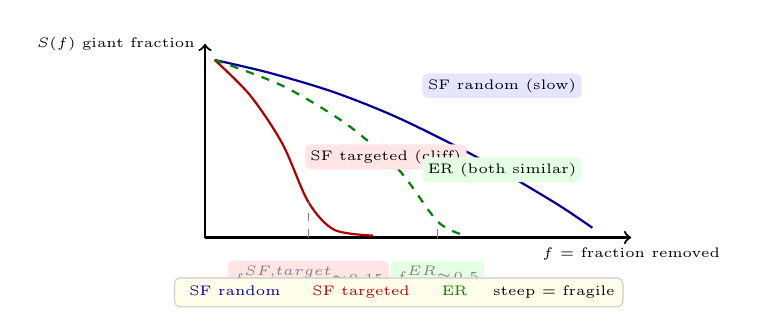
\begin{tikzpicture}[scale=0.82,every node/.style={font=\scriptsize}]
\draw[->,thick] (0,0)--(6.6,0) node[below,font=\tiny] {$f$ = fraction removed};
\draw[->,thick] (0,0)--(0,3.0) node[left,font=\tiny] {$S(f)$ giant fraction};
% random on SF: slow decay
\draw[thick,blue!60!black,smooth] plot coordinates {(0.15,2.75) (1.0,2.55) (2.0,2.25) (3.0,1.85) (4.2,1.25) (5.4,0.55) (6.0,0.15)};
% targeted on SF: cliff
\draw[thick,red!70!black,smooth] plot coordinates {(0.15,2.75) (0.7,2.20) (1.2,1.45) (1.6,0.55) (2.0,0.12) (2.6,0.03)};
% ER random/attack similar
\draw[thick,green!50!black,dashed,smooth] plot coordinates {(0.15,2.75) (1.2,2.35) (2.2,1.75) (3.0,1.05) (3.6,0.25) (4.0,0.04)};
\node[font=\tiny,fill=blue!10,rounded corners=2pt,inner sep=2pt] at (4.6,2.35) {SF random (slow)};
\node[font=\tiny,fill=red!10,rounded corners=2pt,inner sep=2pt] at (2.8,1.25) {SF targeted (cliff)};
\node[font=\tiny,fill=green!10,rounded corners=2pt,inner sep=2pt] at (4.6,1.05) {ER (both similar)};
\draw[dashed,gray] (1.6,0)--(1.6,0.55) node[below,font=\tiny,fill=red!10,rounded corners=2pt,inner sep=2pt] at (1.6,-0.35) {$f_c^{\text{SF,target}}\!\!\approx\!0.15$};
\draw[dashed,gray] (3.6,0)--(3.6,0.25) node[below,font=\tiny,fill=green!10,rounded corners=2pt,inner sep=2pt] at (3.6,-0.35) {$f_c^{\text{ER}}\!\!\approx\!0.5$};
\node[font=\tiny,draw=gray!40,fill=yellow!8,rounded corners=2pt,inner sep=3pt] at (3.0,-0.85) {\textcolor{blue!60!black}{$\blacksquare$ SF random} \quad \textcolor{red!70!black}{$\blacksquare$ SF targeted} \quad \textcolor{green!50!black}{$\blacksquare$ ER} \quad steep = fragile};
\end{tikzpicture}
\caption{Robustness curves $S(f)$. Scale-free (SF) under random removal decays slowly---robust. Under hub-targeted attack it cliffs early ($f_c\approx0.15$)---fragile. ER decays similarly for both (no hubs to target). AUC summarises overall resilience.}
\label{fig:robustness-curves}
\end{figure}

% ============================================================
\section{Percolation Thresholds}
\label{sec:percolation}
\paragraph{Intuition.} Percolation asks: if each node is occupied with probability $p$ (kept with $p$, removed with $1-p$), when does a spanning (giant) cluster appear? The answer depends on moments of $P(k)$.

\begin{theorem}[Molloy--Reed criterion and $p_c$]\label{thm:percolation}
A random graph with degree distribution $P(k)$ has a giant component iff $\langle k^2\rangle/\langle k\rangle>2$. Under random occupation with probability $p$, the threshold is
\begin{equation}
p_c=\frac{\langle k\rangle}{\langle k^2\rangle-\langle k\rangle},\qquad
f_c=1-p_c=1-\frac{\langle k\rangle}{\langle k^2\rangle-\langle k\rangle}.
\end{equation}
For ER with $\langle k\rangle$, $\langle k^2\rangle=\langle k\rangle^2+\langle k\rangle$, so $p_c=1/\langle k\rangle$ and $f_c=1-1/\langle k\rangle$ (e.g.\ $\langle k\rangle=4\Rightarrow f_c=0.75$ for random removal, but only for ER). For scale-free $2<\gamma<3$, $\langle k^2\rangle$ diverges, so $p_c\to0$: the giant survives almost any random removal.
\end{theorem}
\begin{proof}[Idea]
Branching-process as in Ch.~4 but with occupation: following a random edge, the expected number of new occupied neighbours is $p(\langle k^2\rangle/\langle k\rangle-1)$. Giant exists when this exceeds 1, giving $p_c$. \qed
\end{proof}

\begin{figure}[h]\centering
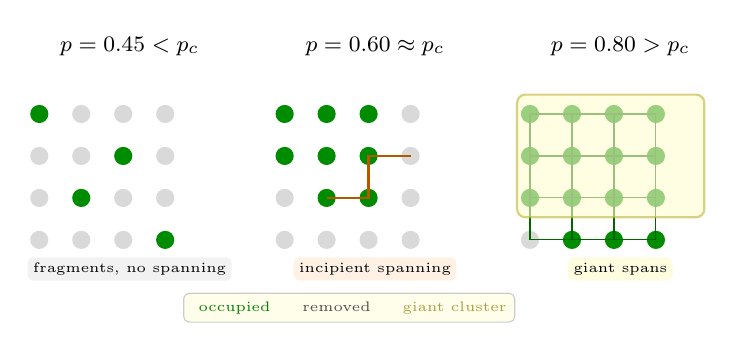
\begin{tikzpicture}[scale=0.82,every node/.style={font=\scriptsize}]
% percolation grid 4x4
\begin{scope}
\node[font=\footnotesize\bfseries] at (1.4,3.0) {$p=0.45<p_c$};
\foreach \x in {0,...,3} \foreach \y in {0,...,3} {
\pgfmathsetmacro{\isocc}{(\x==1&&\y==1)||(\x==2&&\y==2)||(\x==0&&\y==3)||(\x==3&&\y==0) ? 1 : 0}
\ifnum\isocc=1 \fill[green!55!black] (\x*0.65, \y*0.65) circle (4pt);
\else \fill[gray!30] (\x*0.65, \y*0.65) circle (4pt); \fi}
\draw[thick,green!50!black] (0.65,1.95)--(0.65,1.95); % isolated
\node[font=\tiny,fill=gray!10,rounded corners=2pt,inner sep=2pt] at (1.4,-0.45) {fragments, no spanning};
\end{scope}
\begin{scope}[xshift=3.8cm]
\node[font=\footnotesize\bfseries] at (1.4,3.0) {$p=0.60\approx p_c$};
\foreach \x in {0,...,3} \foreach \y in {0,...,3} {
\pgfmathsetmacro{\isocc}{(\x<3&&\y>0) && !(\x==0&&\y==1) ? 1 : 0}
\ifnum\isocc=1 \fill[green!55!black] (\x*0.65, \y*0.65) circle (4pt);
\else \fill[gray!30] (\x*0.65, \y*0.65) circle (4pt); \fi}
\draw[thick,orange!70!black,line width=0.9pt] (0.65,0.65)--(1.30,0.65)--(1.30,1.30)--(1.95,1.30);
\node[font=\tiny,fill=orange!10,rounded corners=2pt,inner sep=2pt] at (1.4,-0.45) {incipient spanning};
\end{scope}
\begin{scope}[xshift=7.6cm]
\node[font=\footnotesize\bfseries] at (1.4,3.0) {$p=0.80>p_c$};
\foreach \x in {0,...,3} \foreach \y in {0,...,3} {
\pgfmathsetmacro{\isocc}{(\x==0&&\y==0) ? 0 : 1}
\ifnum\isocc=1 \fill[green!55!black] (\x*0.65, \y*0.65) circle (4pt);
\else \fill[gray!30] (\x*0.65, \y*0.65) circle (4pt); \fi}
\foreach \x in {0,...,2} \foreach \y in {0,...,3} \draw[thin,green!40!black] (\x*0.65,\y*0.65)--(\x*0.65+0.65,\y*0.65);
\foreach \x in {0,...,3} \foreach \y in {0,...,2} \draw[thin,green!40!black] (\x*0.65,\y*0.65)--(\x*0.65,\y*0.65+0.65);
% highlight giant yellow
\draw[thick,yellow!70!black,rounded corners=3pt,fill=yellow!18,opacity=0.6] (-0.2,0.35) rectangle (2.7,2.25);
\node[font=\tiny,fill=yellow!12,rounded corners=2pt,inner sep=2pt] at (1.4,-0.45) {giant spans};
\end{scope}
\node[font=\tiny,draw=gray!40,fill=yellow!8,rounded corners=2pt,inner sep=3pt] at (4.8,-1.05) {\textcolor{green!50!black}{$\blacksquare$ occupied} \quad \textcolor{gray!60!black}{$\blacksquare$ removed} \quad \textcolor{yellow!60!black}{$\blacksquare$ giant cluster}};
\end{tikzpicture}
\caption{Site percolation on a 2-D lattice. Below $p_c$ only small clusters (left); near $p_c$ a fragile spanning cluster appears (middle); above $p_c$ the giant dominates (right, yellow). Network percolation is the irregular-graph analogue.}
\label{fig:percolation-lattice}
\end{figure}

% ============================================================
\section{Robust Yet Fragile and Hardening}
\label{sec:hardening}
Scale-free networks are \emph{robust yet fragile} (Doyle): random removal likely hits leaves ($f_c\approx1$), but removing a few hubs collapses the giant. ER, with no hubs, treats random and targeted similarly.

Hardening strategies: (i) \emph{onion structure}: sort nodes by degree, link high-degree nodes in layers so the core survives hub removal; (ii) \emph{redundancy / bypass}: add edges that shortcut hubs; (iii) \emph{modular hardening}: reinforce inter-module bridges (Ch.~3) rather than just hubs, since bridges control $S(f)$ when communities are strong.

\begin{figure}[h]\centering
\begin{tikzpicture}[scale=0.82,every node/.style={font=\scriptsize}]
% fragile hub-centric
\begin{scope}
\node[font=\footnotesize\bfseries] at (1.4,2.6) {Fragile (hub)};
\node[circle,draw,thick,fill=red!18,minimum size=0.75cm] (h) at (1.4,1.3) {H};
\foreach \a in {0,45,90,135,180,225,270,315} {\node[circle,draw,fill=blue!10,minimum size=0.48cm] at ($(h)+(\a:1.05)$) {}; \draw[thick] (h)--($(h)+(\a:1.05)$);}
\node[font=\tiny,fill=red!10,rounded corners=2pt,inner sep=2pt] at (1.4,-0.25) {one hit disconnects};
\end{scope}
% onion robust
\begin{scope}[xshift=4.6cm]
\node[font=\footnotesize\bfseries] at (1.6,2.6) {Robust (onion)};
\foreach \r/\c in {0.45/red!18,0.85/orange!16,1.25/blue!12} \draw[thick,fill=\c,opacity=0.7] (1.6,1.1) circle (\r);
\node[circle,draw,thick,fill=red!18,minimum size=0.62cm] at (1.6,1.1) {C};
\foreach \a in {30,90,150,210,270,330} {\node[circle,draw,fill=orange!12,minimum size=0.42cm] at ($(1.6,1.1)+(\a:0.85)$) {}; }
\foreach \a in {0,60,120,180,240,300} {\node[circle,draw,fill=blue!10,minimum size=0.38cm] at ($(1.6,1.1)+(\a:1.25)$) {};}
\draw[thick,gray!50] (1.6,1.1) circle (0.85); \draw[thick,gray!50] (1.6,1.1) circle (1.25);
\node[font=\tiny,fill=green!10,rounded corners=2pt,inner sep=2pt] at (1.6,-0.25) {layers share load};
\end{scope}
% interdependent schematic
\begin{scope}[xshift=8.8cm]
\node[font=\footnotesize\bfseries] at (1.4,2.6) {Interdependent};
\node[circle,draw,thick,fill=blue!15,minimum size=0.55cm] (p1) at (0.5,1.5) {P};
\node[circle,draw,thick,fill=blue!15,minimum size=0.55cm] (p2) at (1.8,1.7) {P};
\node[circle,draw,thick,fill=blue!15,minimum size=0.55cm] (p3) at (1.4,0.7) {P};
\draw[thick,blue!60!black] (p1)--(p2)--(p3)--(p1);
\node[circle,draw,thick,fill=orange!15,minimum size=0.55cm] (q1) at (0.5,0.15) {C};
\node[circle,draw,thick,fill=orange!15,minimum size=0.55cm] (q2) at (1.8,0.35) {C};
\node[circle,draw,thick,fill=orange!15,minimum size=0.55cm] (q3) at (2.3,1.0) {C};
\draw[thick,orange!60!black] (q1)--(q2)--(q3);
\draw[thick,red!70!black,dashed] (p1)--(q1); \draw[thick,red!70!black,dashed] (p2)--(q2);
\node[font=\tiny,fill=red!10,rounded corners=2pt,inner sep=2pt] at (1.4,-0.55) {coupled: one fails both};
\end{scope}
\node[font=\tiny,draw=gray!40,fill=yellow!8,rounded corners=2pt,inner sep=3pt] at (5.2,-0.85) {\textcolor{red!60!black}{$\blacksquare$ hub} \quad \textcolor{orange!60!black}{$\blacksquare$ onion layers} \quad \textcolor{blue!60!black}{$\blacksquare$ power} \quad \textcolor{orange!70!black}{$\blacksquare$ cyber}};
\end{tikzpicture}
\caption{Left: hub-centric is fragile. Middle: onion (concentric degree layers) is hardened---core survives. Right: interdependent networks (power $P$ + cyber $C$, dashed dependencies) cascade: one failure propagates back and forth.}
\label{fig:onion-interdepend}
\end{figure}

\paragraph{Cascades and interdependence.} In a power grid, a line failure redistributes load and can overload neighbours (cascade). In coupled networks (power + communication, Fig.~\ref{fig:onion-interdepend} right), a power node needs a cyber node to operate and vice versa. Buldyrev et~al.\ (2010) showed the percolation becomes first-order (abrupt, discontinuous)---far more catastrophic than single-network second-order decay.

\begin{lstlisting}[language=Python, caption={Robustness curves: random vs hub-targeted removal on BA vs ER.}, label={lst:robustness}]
import networkx as nx
import random

def robustness_curve(G, order):
    H = G.copy(); n = G.number_of_nodes()
    giants = []
    for v in order:
        if v in H: H.remove_node(v)
        if not H: giants.append(0); break
        giant = max(len(c) for c in nx.connected_components(H))
        giants.append(giant / n)
    return giants

G_sf = nx.barabasi_albert_graph(200, 3, seed=0)
G_er = nx.erdos_renyi_graph(200, 0.03, seed=0)
random.seed(0)
for name, G in [("BA", G_sf), ("ER", G_er)]:
    rand_order = random.sample(list(G.nodes()), 50)
    hub_order = sorted(G.degree, key=lambda x: x[1], reverse=True)
    hub_order = [v for v,_ in hub_order[:50]]
    r = robustness_curve(G, rand_order)
    h = robustness_curve(G, hub_order)
    print(f"{name} S after 20 removals: random {r[19]:.2f} targeted {h[19]:.2f}")
\end{lstlisting}

\begin{lstlisting}[language=Python, caption={Percolation threshold check via moment formula.}, label={lst:percolation-moment}]
import networkx as nx
import numpy as np

def percolation_stats(G):
    degs = np.array([d for _, d in G.degree()])
    k1, k2 = degs.mean(), (degs**2).mean()
    pc = k1 / (k2 - k1) if k2 > k1 else 1.0
    return k1, k2, pc, 1-pc

for name, G in [("ER  p=0.03", nx.erdos_renyi_graph(200,0.03,seed=1)),
                ("BA  m=3",   nx.barabasi_albert_graph(200,3,seed=1))]:
    k1,k2,pc,fc = percolation_stats(G)
    print(f"{name}: <k>={k1:.1f} <k2>={k2:.1f} pc={pc:.3f} fc={fc:.3f}"
          f"  robust-random? {fc>0.8}")
\end{lstlisting}

% ============================================================
\section{Chapter Notes}
Albert, Jeong, and Barab\'asi (2000, \emph{Nature}) first demonstrated robust-yet-fragile on the Web and Internet. Cohen et~al.\ (2000, 2001) derived $p_c$ for scale-free nets. Schneider et~al.\ (2011) introduced onion hardening. Buldyrev et~al.\ (2010) discovered first-order percolation in interdependent networks, reshaping infrastructure-risk thinking. For design, Valente--Latora--Marchiori efficiency and Schneider's $R$ index complement $S(f)$.

% ============================================================
\section{Exercises}
\label{sec:ch07-exercises}
\begin{enumerate}[label=E7.\arabic*, leftmargin=*, itemsep=0.8em]
    \item \textbf{Handshake percolation.} For ER with $n=1000$, $\langle k\rangle=4$, compute $p_c$ and $f_c$ for random site percolation. Simulate random removal of $f=0.2,0.5,0.7$ fractions (20 trials each) and report mean $S(f)$. Where does the giant vanish?
    \item \textbf{Hub targeting.} On BA($n=300$, $m=2$) remove the top 10 hubs vs 10 random nodes (10 trials for random). Report mean $S$ after removal. Repeat for ER($n=300$, $p=0.013$) with same $\langle k\rangle$. Which contrast is larger and why?
    \item \textbf{Moment formula.} Given degree sequence $[1,1,1,2,2,2,6,6]$, compute $\langle k\rangle$, $\langle k^2\rangle$, and $p_c$ via the moment formula. Does a giant exist at $p=1$? At $p=0.5$?
    \item \textbf{Onion gain.} Starting from BA(200,3), add 20 ``onion'' edges linking high-degree nodes in layers (pair the top 10 hubs in a cycle, then next 10). Re-measure $S(f)$ under targeted attack ($f=0.1$). Does the hardened network retain a larger giant? By how much?
    \item \textbf{Cascade sketch.} Two coupled ER graphs (100 nodes each, $p=0.04$) with one-to-one dependency (power $i$ depends on cyber $i$). Simulate: remove 10 random power nodes, then alternately prune nodes that lack a giant connection or a live dependency. Report final surviving fraction. Compare to single-network removal of 10 nodes.
\end{enumerate}
% End of Chapter 7
